The characterization of uncladded BCF-12 fibers from Saint-Gobain, which are the fibers selected for the TRITIUM monitor, is described in this section. These fibers are compared to single clad and multiclad BCF-12 fibers to quantify the influence of the clad on their photon collection efficiency. Although commercial clads are too thick for tritium measurements, a sufficiently thin clad could be obtained by vapor deposition. The only difference between these three types of fibers is that uncladded fibers consist of a polystyrene core with a refractive index of $1.60$, whereas single clad fibers have a PMMA clad of $30~\mu\meter$ thickness and a refractive index of $1.49$. Multiclad fibers have a second fluor-acrylic clad of $10~\mu\meter$ thickness  and a refractive index of 1.42. The characterization was carried out for individual scintillating fibers and consisted in a comparative study of the fiber response. To determine the photon collection efficiency, the rate of photons reaching the active area of the photosensor was measured for the different type of fibers. A calibrated Hamamatsu R8520-06SEL PMT with $QE=29.76\%$ quantum efficiency at $\lambda=420~\nano\meter$ was employed. The photon rate $R_{\gamma}$ reaching the photocathode was calculated from,
\begin{equation}
R_{\gamma} = \frac{\left( I_{PMT} - I_{DC} \right)}{q_e \cdot{} QE \cdot{} CE}
\label{eq:NumPhotonsFromIntensityPMT}
\end{equation}
where $I_{PMT}$ is the output current of the PMT, $I_{DC}$ is the dark current, the photoelectron collection efficiency $CE$ and $q_e$ is the electron charge. A simplified scheme of the setup is shown in Figure \ref{fig:SetUpFiberCharacterization}.
\begin{figure}[h]
\centering
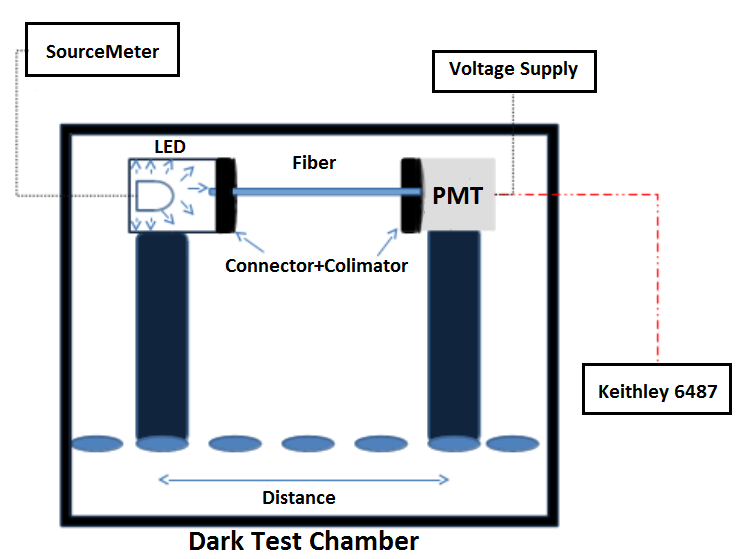
\includegraphics[scale=0.6]{4ResearchAndDevelopments/41Fibers/SetUp_Fiber_Characterization.png}
\caption{Setup used for fiber characterization.\label{fig:SetUpFiberCharacterization}}
\end{figure}
This setup consists of an optical board on which a LED and a PMT were placed in front of each other. A LED (LED435-03 from Roithner LaserTechnik Gmbh \cite{LEDRLT}), with an emission spectrum similar to that of the scintillating fibers, was used. The emission spectrum of the LED, given in Figure \ref{fig:LEDSpectrumTritium}, was measured using a spectrometer and fitted to a Gaussian function. The LED emission peak is at $434~\nano\meter$ with a $\sigma$ of $8~\nm$. The LED was fed in current mode with a sourcemeter. A fiber of $20~\cm$ long was placed between the LED and the PMT, optically coupled to their end-surfaces by optical grease \cite{OpticalGrease}. Two collimators were used to ensure that only photons emitted from the LED were detected by the PMT. Two FH-ST connectors from RoHS \cite{} were used to fasten the fiber to the system. 

\begin{figure}[h]
\centering
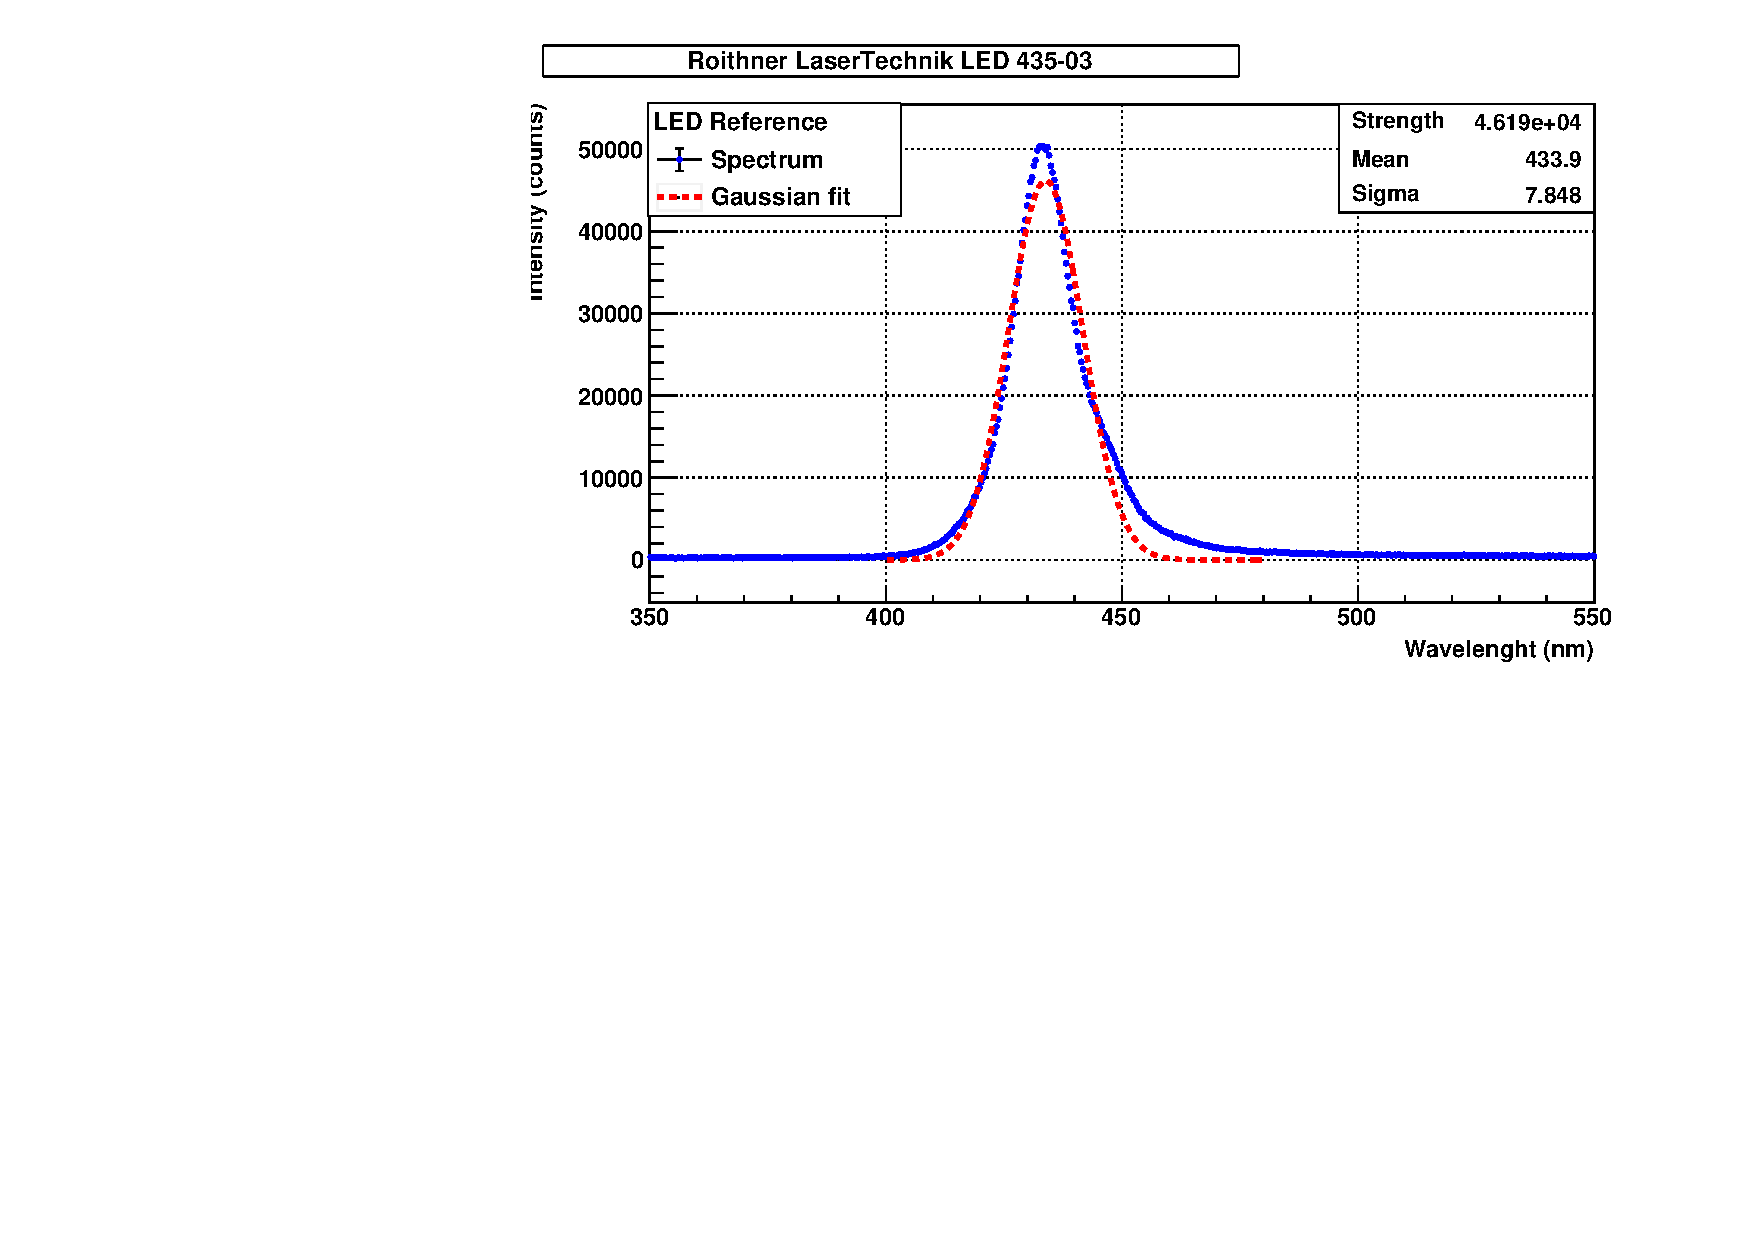
\includegraphics[scale=0.6]{4ResearchAndDevelopments/41Fibers/LED_TRITIUM_1_std.pdf}
\caption{Emission spectrum mesured for the 435-03 LED from Roithner LaserTechnik Gmbh.\label{fig:LEDSpectrumTritium}}
\end{figure}